% This file was created with tikzplotlib v0.10.1.
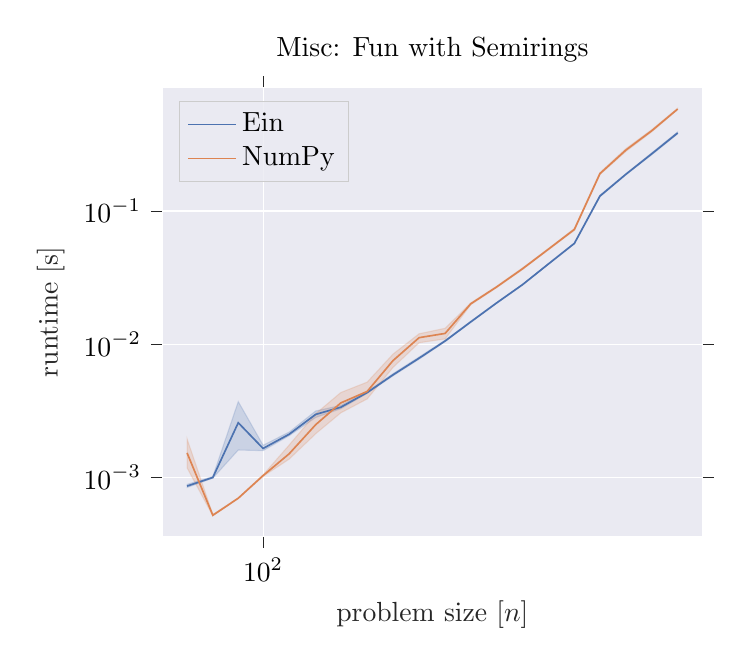
\begin{tikzpicture}

\definecolor{darkslategray38}{RGB}{38,38,38}
\definecolor{lavender234234242}{RGB}{234,234,242}
\definecolor{lightgray204}{RGB}{204,204,204}
\definecolor{peru22113282}{RGB}{221,132,82}
\definecolor{steelblue76114176}{RGB}{76,114,176}

\begin{axis}[
axis background/.style={fill=lavender234234242},
axis line style={white},
legend cell align={left},
legend style={
  fill opacity=0.8,
  draw opacity=1,
  text opacity=1,
  at={(0.03,0.97)},
  anchor=north west,
  draw=lightgray204,
  fill=lavender234234242
},
log basis x={10},
log basis y={10},
tick align=outside,
title={Misc: Fun with Semirings},
x grid style={white},
xlabel=\textcolor{darkslategray38}{problem size \(\displaystyle [n]\)},
xmajorgrids,
xmajorticks=true,
xmin=62.3875656693622, xmax=785.412918011374,
xmode=log,
xtick style={color=darkslategray38},
xtick={1,10,100,1000,10000},
xticklabels={
  \(\displaystyle {10^{0}}\),
  \(\displaystyle {10^{1}}\),
  \(\displaystyle {10^{2}}\),
  \(\displaystyle {10^{3}}\),
  \(\displaystyle {10^{4}}\)
},
y grid style={white},
ylabel=\textcolor{darkslategray38}{runtime \(\displaystyle [\mathrm{s}]\)},
ymajorgrids,
ymajorticks=true,
ymin=0.000360273084941951, ymax=0.840756866074562,
ymode=log,
ytick style={color=darkslategray38},
ytick={1e-05,0.0001,0.001,0.01,0.1,1,10},
yticklabels={
  \(\displaystyle {10^{-5}}\),
  \(\displaystyle {10^{-4}}\),
  \(\displaystyle {10^{-3}}\),
  \(\displaystyle {10^{-2}}\),
  \(\displaystyle {10^{-1}}\),
  \(\displaystyle {10^{0}}\),
  \(\displaystyle {10^{1}}\)
}
]
\path [draw=steelblue76114176, fill=steelblue76114176, opacity=0.2]
(axis cs:70,0.000882980736569152)
--(axis cs:70,0.000836469603709702)
--(axis cs:79,0.000983666491465556)
--(axis cs:89,0.00160017079695535)
--(axis cs:100,0.00158288053147771)
--(axis cs:113,0.00204948378828703)
--(axis cs:128,0.00280844490238451)
--(axis cs:144,0.00326712702590157)
--(axis cs:163,0.00426672655372386)
--(axis cs:184,0.00577486806374509)
--(axis cs:208,0.00770885239919153)
--(axis cs:235,0.0104360073216048)
--(axis cs:265,0.0145424592601194)
--(axis cs:299,0.0201871005468638)
--(axis cs:338,0.0277885871910621)
--(axis cs:381,0.0395295096395785)
--(axis cs:431,0.0567088302808366)
--(axis cs:486,0.127795878605548)
--(axis cs:549,0.187310844089916)
--(axis cs:620,0.264747474796604)
--(axis cs:700,0.379321700398577)
--(axis cs:700,0.392475692002336)
--(axis cs:700,0.392475692002336)
--(axis cs:620,0.273306374798995)
--(axis cs:549,0.190437548428054)
--(axis cs:486,0.131277720707976)
--(axis cs:431,0.0574690455018653)
--(axis cs:381,0.0400586240080884)
--(axis cs:338,0.0281631004092378)
--(axis cs:299,0.0204711578140632)
--(axis cs:265,0.0148268214958807)
--(axis cs:235,0.0106902608964265)
--(axis cs:208,0.00799688121056533)
--(axis cs:184,0.00599107745618312)
--(axis cs:163,0.0043952521038409)
--(axis cs:144,0.00346288692931921)
--(axis cs:128,0.00314344688005804)
--(axis cs:113,0.00217874632706298)
--(axis cs:100,0.00173873103536607)
--(axis cs:89,0.00369602308688627)
--(axis cs:79,0.00101039469656826)
--(axis cs:70,0.000882980736569152)
--cycle;

\path [draw=peru22113282, fill=peru22113282, opacity=0.2]
(axis cs:70,0.00193848101255118)
--(axis cs:70,0.00117677244190284)
--(axis cs:79,0.000512536126241976)
--(axis cs:89,0.000691374327275463)
--(axis cs:100,0.00101480922461673)
--(axis cs:113,0.0013658054360003)
--(axis cs:128,0.00212054063949876)
--(axis cs:144,0.00304233388874813)
--(axis cs:163,0.00387155986232424)
--(axis cs:184,0.00667547516394288)
--(axis cs:208,0.0102306443561746)
--(axis cs:235,0.0109339212095422)
--(axis cs:265,0.019764288904906)
--(axis cs:299,0.0264826368818243)
--(axis cs:338,0.0363230633929786)
--(axis cs:381,0.0508596943735536)
--(axis cs:431,0.0714440472078674)
--(axis cs:486,0.187855203689419)
--(axis cs:549,0.280232980105275)
--(axis cs:620,0.393550276078777)
--(axis cs:700,0.577770442721567)
--(axis cs:700,0.590986770138042)
--(axis cs:700,0.590986770138042)
--(axis cs:620,0.408690926201109)
--(axis cs:549,0.293886953764823)
--(axis cs:486,0.194362045148285)
--(axis cs:431,0.0738519055358364)
--(axis cs:381,0.0519194425429355)
--(axis cs:338,0.0373699798928444)
--(axis cs:299,0.0271283243346789)
--(axis cs:265,0.020363228674962)
--(axis cs:235,0.0131407148729523)
--(axis cs:208,0.0119519829952601)
--(axis cs:184,0.00840683975339437)
--(axis cs:163,0.00517817608230361)
--(axis cs:144,0.00432445873980756)
--(axis cs:128,0.00299782580115713)
--(axis cs:113,0.00174265249451506)
--(axis cs:100,0.00104073359240367)
--(axis cs:89,0.000698650182437273)
--(axis cs:79,0.000523782635826371)
--(axis cs:70,0.00193848101255118)
--cycle;

\addplot [semithick, steelblue76114176]
table {%
70 0.000857760399958352
79 0.000994293649273459
89 0.00256512295018183
100 0.00164436434788513
113 0.00210113954890403
128 0.00296312304708408
144 0.00335419795010239
163 0.00432160414857208
184 0.00587280215040664
208 0.0078401249491435
235 0.0105500666497392
265 0.0146726103506808
299 0.0203304040995135
338 0.027970593853388
381 0.0397933979991649
431 0.0570397616684204
486 0.129457755250769
549 0.188722222330398
620 0.269026924797799
700 0.38559165839979
};
\addlegendentry{Ein}
\addplot [semithick, peru22113282]
table {%
70 0.00152205276548332
79 0.000517646586514327
89 0.000694967112294748
100 0.00102787029947846
113 0.00149808545271352
128 0.00247987456241484
144 0.00361289884685628
163 0.00440781469366663
184 0.00751455303028802
208 0.0111746290230265
235 0.0120248630362191
265 0.020062592361727
299 0.0268113644896092
338 0.0368154788839337
381 0.0513946486001272
431 0.0726436004298779
486 0.190808159953479
549 0.286831809215619
620 0.401049157632001
700 0.583262162683683
};
\addlegendentry{NumPy}
\end{axis}

\end{tikzpicture}
